\documentclass[12pt,letterpaper]{article}

% ---------- Packages ----------
\usepackage[letterpaper,margin=1in]{geometry}
\usepackage[T1]{fontenc}
\usepackage[utf8]{inputenc}
\usepackage{newtxtext,newtxmath} % Times-like font
\usepackage{microtype}
\usepackage{graphicx}
\usepackage{booktabs}
\usepackage{array}
\usepackage{tabularx}
\usepackage{enumitem}
\usepackage{titlesec}
\usepackage{xcolor}
\usepackage{hyperref}
\usepackage{fancyhdr}

% ---------- Colors (from Aspose export) ----------
\definecolor{brand}{rgb}{0.478431,0,0.235294}   % color_147093
\definecolor{accent}{rgb}{0.67451,0.078431,0.333333} % color_195788
\definecolor{textgray}{rgb}{0.2,0.2,0.2}        % color_80434
\definecolor{rulegray}{rgb}{0.866667,0.866667,0.866667} % color_249244

% ---------- Document styling ----------
\hypersetup{colorlinks=true,linkcolor=brand,urlcolor=accent,citecolor=brand}
\pagestyle{fancy}
\fancyhf{}
\lhead{}
\rhead{}
\lfoot{SE/CS 3RA3 — Fall}
\rfoot{\thepage}
\renewcommand{\headrulewidth}{0pt}
\renewcommand{\footrulewidth}{0.4pt}

\titleformat{\section}{\Large\bfseries\color{brand}}{\thesection}{0.75em}{}
\titleformat{\subsection}{\large\bfseries\color{brand}}{\thesubsection}{0.75em}{}
\titleformat{\subsubsection}{\normalsize\bfseries\color{brand}}{\thesubsubsection}{0.75em}{}

\setlist[itemize]{topsep=4pt,itemsep=2pt,parsep=0pt}
\setlist[enumerate]{topsep=4pt,itemsep=2pt,parsep=0pt}

% ---------- Title page ----------
\makeatletter
\def\@maketitle{%
  \begin{center}
    \vspace*{1.5cm}
    {\Huge\bfseries\color{brand} Our Awesome Project\par}
    \vspace{0.35cm}
    {\Large\itshape\color{accent} Requirements Standard Plan\par}
    \vspace{0.9cm}
    {\large Saad Salman, Author 2, Author 3\par}
    \vspace{0.25cm}
    {\normalsize Version 1, 2025-09-22\par}
    \vspace{1.5cm}
  \end{center}
}
\makeatother
\title{}
\author{}
\date{}

\begin{document}
\maketitle
\thispagestyle{empty}
\clearpage

\tableofcontents
\clearpage

% ---------- Academic Integrity Disclaimer ----------
\section*{Academic Integrity Disclaimer}
\addcontentsline{toc}{section}{Academic Integrity Disclaimer}
We would like to acknowledge that as dedicated students of McMaster University, we have thoroughly read and comprehended the Academic Integrity Policy published by the university. We are committed to upholding the principles of academic honesty and integrity in all aspects of our educational journey. We understand the importance of acknowledging the work and ideas of others, and we pledge to ensure that all our academic endeavors are conducted with the utmost originality and compliance with the university's policy.

We affirm that the content presented in this document is entirely our own, and any external sources used have been appropriately cited and referenced.

\medskip
\noindent\textbf{Saad Salman} \\
As I submit my work, I, Saad Salman, take full responsibility for the integrity of my work and promise to avoid any form of plagiarism, cheating, or dishonest behavior. This acknowledgment serves as a testament to my dedication to academic excellence and the fostering of a trustworthy academic community at McMaster University.

\medskip
\noindent\textbf{Author 2} \\
As I submit my work, I, Author 2, take full responsibility for the integrity of my work and promise to avoid any form of plagiarism, cheating, or dishonest behavior. This acknowledgment serves as a testament to my dedication to academic excellence and the fostering of a trustworthy academic community at McMaster University.

\medskip
\noindent\textbf{Author 3} \\
As I submit my work, I, Author 3, take full responsibility for the integrity of my work and promise to avoid any form of plagiarism, cheating, or dishonest behavior. This acknowledgment serves as a testament to my dedication to academic excellence and the fostering of a trustworthy academic community at McMaster University.

\medskip
\noindent\textit{Policy:} \url{https://secretariat.mcmaster.ca/app/uploads/Academic-Integrity-Policy-1-1.pdf}

\clearpage

% ---------- Control Information ----------
\section{Control Information}
\begin{table}[h!]\centering
\caption*{Versioning and Delivery}
\renewcommand{\arraystretch}{1.2}
\begin{tabularx}{\textwidth}{@{}l l l l l l@{}}
\toprule
\textbf{Version} & \textbf{Delivery Deadline} & \textbf{Delivered} & \textbf{Feedback Received} & \textbf{Integrated} & \textbf{Notes} \\
\midrule
V1 & & & & & \\
V2 & & & & & \\
V3 & & & & & \\
\bottomrule
\end{tabularx}
\end{table}

\medskip
\noindent\textbf{Saad Salman} \\
Here is a quick biography of Saad Salman. You can contact them at \href{mailto:salmam12@mcmaster.ca}{salmam12@mcmaster.ca}.

\medskip
\noindent\textbf{Author 2} \\
Here is a quick biography of Author 2. You can contact them at \href{mailto:a2@mcmaster.ca}{a2@mcmaster.ca}.

\medskip
\noindent\textbf{Author 3} \\
Here is a quick biography of Author 3. You can contact them at \href{mailto:a3@mcmaster.ca}{a3@mcmaster.ca}.

\clearpage

% ---------- (G) Goals ----------
\section{(G) Goals}
\subsection*{Reading Guide}
Goals are ``needs of the target organization, which the system will address. While the development team is the principal user of the other books, the Goals book addresses a wider audience: essentially, all stakeholders \cite{meyer2022}. It must contain enough information to provide---if read just by itself---a general sketch of the entire project. To this effect, chapter G.3 presents a short overview of the system and G.1 will typically include some key properties of the environment. As it addresses a wide readership, it should be clear and minimize the use of specialized technical terms. Together, G.1, G.2 and G.3 describe the rationale for the project. It is important to state these justifications explicitly. Typically, they are well understood at the start of the project, but management and priorities can change \cite{meyer2022}.

\subsection*{Control Information}
\begin{table}[h!]\centering
\caption*{Table 1. Our Awesome Project --- Versioning Information --- Goal Book}
\renewcommand{\arraystretch}{1.1}
\begin{tabularx}{\textwidth}{@{}l l l l l l@{}}
\toprule
\textbf{Section} & \textbf{Version} & \textbf{Lead} & \textbf{Delivered on} & \textbf{Reviewer} & \textbf{Approved on} \\
\midrule
G.1 & M1 & SS & Sept-21-2025 & SP & Sept-22-2025 \\
G.2 & M1 & SS & Sept-21-2025 & SP & Sept-22-2025 \\
G.3 & & & & & \\
G.4 & & & & & \\
G.5 & & & & & \\
G.6 & & & & & \\
G.7 & & & & & \\
\bottomrule
\end{tabularx}
\end{table}

\subsection{(G.1) Context and Overall Objectives}
High-level view of the project: organizational context and reason for building a system. It explains why the project is needed, recalls the business context, and presents the general business objectives \cite{meyer2022}.

New university students trying to make connections with each other can often find it difficult due to the limited interactions they have outside of their program. \textit{HammerCorp Inc.} will address this by developing a web and mobile app called \textbf{ACME Connect}, which connects students based on similar interests or experiences, as well as student clubs or institutional activities. It aims to improve the overall university experience by creating a tightly-knit student community where integration of official activities happens at the student level. With safety as a primary goal, this project plans to be available to universities across North America, with a pilot program starting at McMaster University.

\subsection{(G.2) Current Situation}
Current state of processes to be addressed by the project and the resulting system. It describes the current situation upon which the system is expected to improve \cite{meyer2022}.

At the moment, students are limited to in-person connections within their program or at Welcome Week events, which are often not sufficient for engagement and networking. Residence and international students may feel disconnected in a new place. Student clubs and associations also find it difficult to engage potential members. Although there are in-person events for new students and club booths around campus, those are temporary pop-ups and may not reach everyone. There is no central place for everyone to connect outside those events. Discord servers exist; however, they are often not institutionally based, which can compromise safety and allow complete strangers not affiliated with the school. Looking at these challenges, \textbf{ACME Connect} plans to address them and create a safe environment for students and institutions to foster lasting relationships throughout the university journey.

\subsection{(G.3) Expected Benefits}
New processes, or improvements to existing processes, made possible by the project's results. It presents the business benefits expected from successful execution of the project. This chapter is the core of the Goals book, describing what the organization expects from the system \cite{meyer2022}.

\textit{Nothing available at this point.}

\subsection{(G.4) Functionality Overview}
Overview of the functions (behavior) of the system. Principal properties only (details are in the System book). A capsule version of book S that enables readers to get a quick grasp of what the system will do \cite{meyer2022}.

\textit{Nothing available at this point.}

\subsection{(G.5) High-level Usage Scenarios}
Fundamental usage paths through the system, stated in user terms and independent of the system's structure. Detailed usage scenarios appear in the System book (S.4) \cite{meyer2022}.

\begin{center}
\fbox{\parbox{0.7\linewidth}{\centering \emph{(High level use case diagram placeholder)}}}
\end{center}

\textit{Nothing available at this point.}

\subsection{(G.6) Limitations and Exclusions}
Aspects that the system need not address; scoping the requirements. (Risks and obstacles belong to P.6.) \cite{meyer2022}.

\textit{Nothing available at this point.}

\subsection{(G.7) Stakeholders and Requirements Sources}
Stakeholder categories that can affect or be affected by the project, and other sources of requirements information \cite{meyer2022}.

\textit{Nothing available at this point.}

\clearpage

% ---------- (E) Environment ----------
\section{(E) Environment}

\subsection{(E.1) Glossary}
\begin{itemize}
\item \textbf{Rideshare:} A service that allows riders to carpool with a single driver to reach a common destination.
\item \textbf{Drivers:} They are users that will provide rideshare services with their personal vehicles.  
\item \textbf{Riders:} They are users that will carpool to and from McMaster University.
\item \textbf{Working Condition:} A vehicle is in working condition if it has all necessary functions in the vehicle working. For instance, it must have functional head/tail lights, tires, engine, brakes, brake lights etc.
\end{itemize}

\begin{figure}[h] 
    \centering
    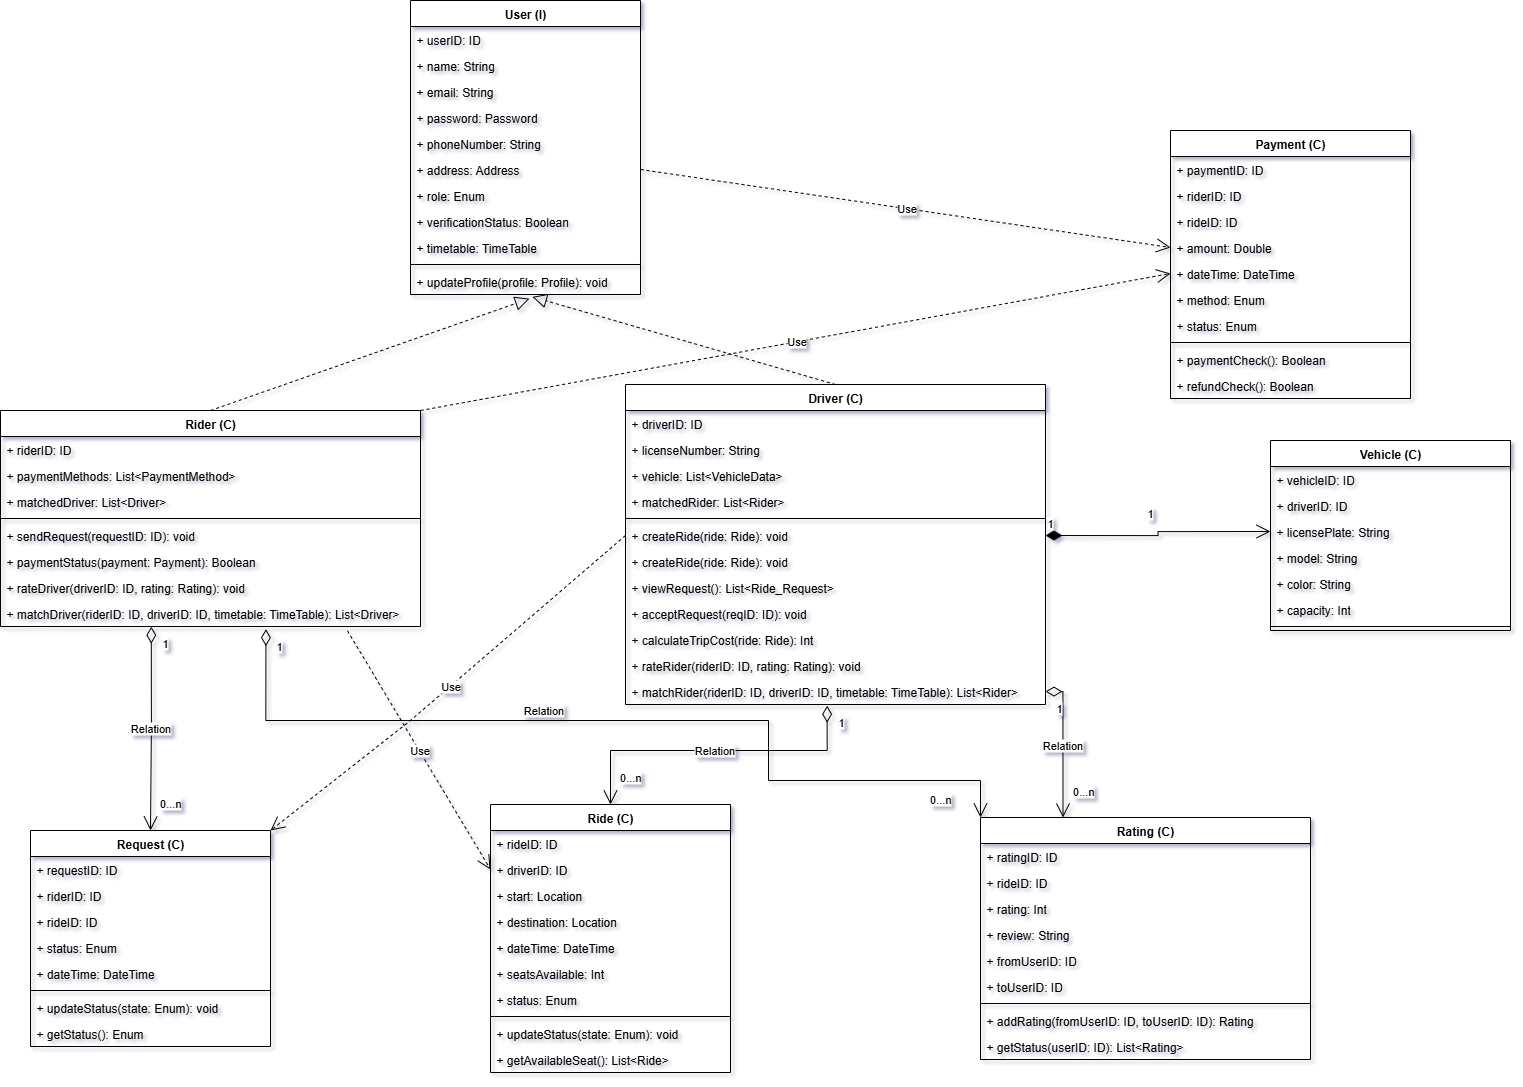
\includegraphics[width=0.8\linewidth]{Domain Model.png}
    \caption{Domain Model}
    \label{fig:domain-model}
\end{figure}

\subsection{(E.2) Components}
\begin{enumerate}
\item \textbf{MFA (Multi-Factored Authentication) Services:} The application will be interacting with components that will allow the application to verify users with their McMaster University emails with SMS/Phone verification. This is to ensure reliability and user trust.
\item \textbf{Payments Interface (i.e, Credit Cards, PayPal, Apple Pay etc.):} The application will also interact with a payment interface to allow for a smooth and streamlined payment process with Stripe. 
\item \textbf{Location API:} Google Maps will be used in several components of the application. This API will be used for location tracking, distance calculations, and for routing.
\end{enumerate}

\subsection{(E.3) Constraints}
These are a few limitations and restrictions coming from the environment onto the system: 
\begin{enumerate}
\item \textbf{Usage Constraint:} The project is currently limited and available to the McMaster community only. This would only include users that are currently students, staff members, or faculty members of the university. This application is currently limited to the Android and IOS operation systems. They will be compatible with any device with this operating system.
\item \textbf{Regulatory Constraint:} The project is constrained to comply with the PIPEDA laws and standards. This ensures that the user's data is handled carefully and with significant attention to maintaining data integrity and security. Each driver must have a Candian issued G2/G license, and the vehicle must be registered and insured. Each driver must comply with Ontario traffic rules and regulations. They must also not exceed the maximum passenger limit for their vehicle.
\item \textbf{Technical Constraints and Limitations:} A limitation of the Google Maps API is that it will be limited to providing minimal data for locations in rural areas. All functionalities in the applications must be completed in a limited time. For instance, the processing time for payments must be minimal. 
\end{enumerate}


\subsection{(E.4) Assumptions}
There are a few important assumptions that will be made to simplify the system. These will be assumed to be held, however, are not explicit constraints in the system.  
\begin{enumerate}
\item \textbf{User Behavior:} All users of the rideshare application will not intentionally cause any harm to each other during a trip. They will not misbehave or litter in the car. This is an important assumption as it ensures the safety of users and simplifies the process of carpooling.  
\item \textbf{Vehicle Condition:} Each driver has a vehicle that is in proper working condition. They are assumed to keep their vehicles clean. It will also be assumed that drivers will regularly maintain their vehicles.
\item \textbf{Language:} All users of the rideshare application must have a basic understanding of the English language, and they are able to communicate their thoughts with each other.
\item \textbf{User Base Demographic:} The application will assume a user base consisting of members of the McMaster University community. This may include students, staff, and faculty. This user group encompasses a diverse range of ages, genders, and ethnicities.
\item \textbf{Technical Compatibility and Reliability:} All third-party applications and API are assumed to be reliable. For instance, the Maps API will provide accurate data for all users in the GTA region. The API's rate limits will not exceed the expected user load. They are also assumed to have minimal downtime. 
\end{enumerate}

\subsection{(E.5) Effects}
Elements and properties of the environment that the system will affect \cite{meyer2022}. Effects of the application include:
\begin{enumerate}
\item \textbf{Improved sustainability and Reduced Traffic Congestion:} The system will positively affect the environment by lowering the GHG emissions caused by vehicles of individuals commuting to and from McMaster University. Secondly, as a result of carpooling, there will be a reduction in the use of single-occupancy vehicles which will cause a reduction in traffic congestion on roads and highways. 
\item \textbf{Usage of Public Transit:} There will be a significant reduction in the usage of buses and trains to commute to McMaster University because of the transition of people moving towards using the rideshare application, Hitchly. It may become convenient and affordable for commuters to use the rideshare services. Thus, resulting in a potential reduction in the usage of public transit.  
\item \textbf{UIncrease in Parking Spaces:} There can be an increase in available parking spaces due to the overall reduction of vehicles arriving at McMaster University. As a result of using the rideshare platform Hitchly, the number of single-occupancy vehicles will decrease. This would mean that fewer cars would arrive at McMaster University, reducing the overall demand for parking spaces.
\item \textbf{Increased Savings:} There can be an overall increase in the amount each commuter saves as a result of shifting to carpooling from other modes of transportation. Carpooling enables users to divide and share their cost, resulting in leaving them with more money in hand. 
\end{enumerate}

\subsection{(E.6) Invariants}
\begin{itemize}
\item Regular traffic will continue to move in Hamilton and surrounding areas where riders and drivers live. There can be traffic congestion on the roads due to car crashes and unusual weather conditions. There will also be times when an emergency vehicle may be on the roads occasionally, causing traffic congestion. These conditions will be present and will not change after the implementation of the application.  
\item The city of Hamilton will have and maintain their city infrastructure. There will be traffic lights, roads highways, pedestrian sidewalks, that will function normally.  The traffic rules and signs will be followed and maintained regardless of the implantation of the application. 
\item McMaster Parking systems will function as usual. There will not be any changes made to the parking rules or guidelines to specifically cater to the rideshare application users. 
\item Wi-Fi networks will operate independently and can become slow due to torrential weather conditions. Users may be affected by this as it can affect their accessibility to a Wi-Fi network during their ride. Lastly, the Wi-Fi networks function independently of the implementation of the application.  
\end{itemize}

\clearpage

% ---------- (S) System ----------
\section{(S) System}
The System book refines the Goals book by focusing on more detailed requirements.

\subsection{(S.1) Components}
Overall structure expressed by the list of major software and, if applicable, hardware parts \cite{meyer2022}.

\textit{Nothing available at this point.}

\subsection{(S.2) Functionality}
The bulk of the System book: functional and non-functional behaviors \cite{meyer2022}.

\textit{Nothing available at this point.}

\subsection{(S.3) Interfaces}
How the system makes S.2 functionality available to the rest of the world (UIs and APIs) \cite{meyer2022}.

\textit{Nothing available at this point.}

\subsection{(S.4) Detailed Usage Scenarios}
User stories and examples of interaction between users/environment and the system \cite{meyer2022}.

\textit{Nothing available at this point.}

\subsection{(S.5) Prioritization}
Classification of behaviors, interfaces, and scenarios by criticality \cite{meyer2022}.

\textit{Nothing available at this point.}

\subsection{(S.6) Verification and Acceptance Criteria}
Conditions under which an implementation will be deemed satisfactory; V\&V levels \cite{meyer2022}.

\textit{Nothing available at this point.}

\clearpage

% ---------- (P) Project ----------
\section{(P) Project}

\subsection{(P.1) Roles and Personnel}
Main responsibilities, required staff, and qualifications \cite{meyer2022}.

\textit{Nothing available at this point.}

\subsection{(P.2) Imposed Technical Choices}
A priori choices binding the project to specific tools, hardware, languages or other technical parameters \cite{meyer2022}.

\textit{Nothing available at this point.}

\subsection{(P.3) Schedule and Milestones}
List of tasks to be carried out and their scheduling \cite{meyer2022}.

\textit{Nothing available at this point.}

\subsection{(P.4) Tasks and Deliverables}
Details of individual tasks and expected outcomes, associated with milestone dates \cite{meyer2022}.

\textit{Nothing available at this point.}

\subsection{(P.5) Required Technology Elements}
External systems, hardware and software expected to be necessary for building the system \cite{meyer2022}.

\textit{Nothing available at this point.}

\subsection{(P.6) Risk and Mitigation Analysis}
Potential obstacles to meeting the schedule and measures for adapting the plan \cite{meyer2022}.

\textit{Nothing available at this point.}

\subsection{(P.7) Requirements Process and Report}
Initially: description of the requirements process; later: report on its steps \cite{meyer2022}.

\textit{Nothing available at this point.}

\clearpage

% ---------- References ----------
\begin{thebibliography}{9}
\bibitem{meyer2022} Bertrand Meyer. \textit{Handbook of Requirements and Business Analysis}. Springer, 2022.
\bibitem{sommerville1997} Ian Sommerville and Peter Sawyer. \textit{Requirements Engineering: A Good Practice Guide}. Wiley, 1997.
\end{thebibliography}

\end{document}